\subsection{Two appearance modules that did not pass}
\label{sec:exp_neg}
% generated by paper_numbers.py: frozen variants from r1full (same front-end pass and evaluation job as Table 1)
\begin{table}[t]
\centering
\caption{\textbf{Two appearance modules that did not pass their pre-registered criteria} (same front-end pass and evaluation job as \cref{tab:main}). $\Delta$App.: paired appearance difference to B1 with 95\% bootstrap CI, on the clips outside both development sets (477 clips); the criterion required the upper bound to be below 0. R1 changed 7 clips, 5 of them development clips.}
\label{tab:reuse}
\setlength{\tabcolsep}{3pt}
\resizebox{\linewidth}{!}{%
\begin{tabular}{@{}lcccc@{}}
\toprule
 & Read.\ $\uparrow$ & Net $\uparrow$ & App.\ $\downarrow$ & $\Delta$App.\ vs.\ B1 \\
\midrule
\method (B1, final) & 91.4 & 198 & 2.57 & -- \\
+ baseline layout + glyph-shape font (B1f) & 91.3 & 197 & 2.61 & $+0.052$ [$+0.002$, $+0.106$] \\
+ source-glyph reuse (R1) & 91.4 & 198 & 2.56 & $+0.021$ [$-0.023$, $+0.067$] \\
+ both (R1f) & 91.3 & 197 & 2.57 & $+0.034$ [$-0.016$, $+0.092$] \\
\bottomrule
\end{tabular}}
\end{table}


Two of the causes of the appearance gap (\cref{sec:limits}) look addressable without generation: the new text ignores the orientation and the typeface of the old one, and the garbled source already contains most of the target's letters. We built one module for each and fixed their acceptance criteria before running them on the benchmark (supplement). Both were run in the same front-end pass and evaluation job as \cref{tab:main}, so every comparison in \cref{tab:reuse} is paired.

\paragraph{Baseline-aligned layout and glyph-matched fonts (B1f).} The first component lays the new text along the baseline of the old glyphs instead of the axis-aligned OCR quad, when two ink-based angle estimates agree within $2^\circ$ and the rotation lies between $2^\circ$ and $20^\circ$. The second chooses the typeface by the shapes of the source letters whose identity can be established---the multi-frame consensus reading aligned to the target---and replaces the matched font only if the best per-letter overlap is at least 0.6 (English, single row). The criteria were: readability at most one point lower, a paired appearance difference whose 95\% CI lies below zero, and perceived naturalness not worse in a later human study. The text was rotated in \rTiltN{} clips and the font replaced in \rFshapeN; elsewhere the output equals B1. Readability is unchanged (0 vs.\ 1 discordant clips), but the appearance difference is $\rBOnefMadDiffND$ [$\rBOnefMadLoND$, $\rBOnefMadHiND$] on the clips outside both development sets, so the second criterion is not met and B1f is not adopted. Under the current evaluation protocol we observe no overall benefit; its perceptual effect has not been verified. We do not read this as evidence that font or orientation alignment is ineffective, for two reasons. First, the appearance distance is glyph-agnostic by construction (colour, contrast, halo, edge softness and shading inside the strokes, \cref{sec:metrics}): it does not see typeface similarity or text orientation, which are exactly what B1f changes. Choosing it as the criterion for these components was an error in our pre-registration, which we report rather than amend after the fact. Second, the distance is not deterministic: its ink segmentation runs $k$-means with random initialisation, and on the \rRetestN{} clips where R1 leaves the output byte-identical to B1, the two scores agree exactly in only \rRetestSame{} clips, differ with a standard deviation of \rRetestSD{} per clip, and differ by $\rRetestMean$ [$\rRetestLo$, $\rRetestHi$] on average. B1f's difference is of the same order as this test--retest noise. Deciding whether B1f looks better requires its own pre-registered human study.

\paragraph{Source-glyph reuse (R1).} R1 keeps the source letters that are already correct in place---with their own pixels, font, material and perspective---erases only the wrong span between them, and renders only the missing letters, in a font chosen to match the kept ones. It acts only when the evidence is strong: the number of segmented source letters equals the reading, at least half of the target letters are kept, the kept letters are read stably across frames, no letter must be inserted or deleted between kept letters, the new letters' shapes match the kept ones (overlap at least 0.65), and the new text stays on its carrier; otherwise the clip keeps the B1 output. R1 was applied to \rReuseApplied{} of the 526 clips (\rReuseGarbledEn{} of the \rGarbledEn{} garbled English clips), \rReuseAppliedDev{} of them development clips. On the two others the appearance distance improved by \rReuseNDMad{} with unchanged readability, which is far too few clips to evaluate the criteria. The limiting factor is coverage: in \rReuseWhyLetters{} English clips the segmented letters did not match the reading, in \rReuseWhySource{} the pipeline's consensus reading of the source already equalled the target, and in \rReuseWhyFont{} no font matched the kept letters well enough. With our current letter segmentation, matching and gating, reuse applies to too few clips to form a general module. This bounds the implementation, not the idea; the 20\% coverage observed on a 30-clip sample before the full run did not hold on the benchmark.

Both modules are frozen and are not part of \method, which in \cref{tab:main} is B1.

\paragraph{Reconstruction without source glyphs.} \method's evidence gating assumes that some glyph survives. Classifying the benchmark with the frozen localiser (supplement), \lthreeGlyphs{} clips have readable matches, \lthreeLtwo{} have detectable but unreadable pseudo-text, and none lacks a detectable text-like region; \method reads \lthreeLtwoBoneRead\% of the pseudo-text clips through its detection-box fallback (\steer: \lthreeLtwoSteerRead\%). We additionally investigated glyph-free, carrier-conditioned text reconstruction, which lays the target out from the tracked carrier alone, with no glyph mask, OCR box or letter height. The first registered branch, evaluated on the \lthreeGlyphs{} clips with their glyphs erased, read \lthreeACarRead\% of the locatable clips where the frozen code's static-hint fallback reads \lthreeABfbRead\%, but missed the registered geometry and stability criteria (\lthreeAPassed{} of \lthreeACriteria); two further registered rounds also failed (\cref{sec:supp_g_rounds}). A fourth version, designed on a separate development set, was frozen and evaluated once on a sealed set of clips from two other generators (CogVideoX-5B and Wan2.2-TI2V-5B; \gTSynN{} glyph-erased clips with geometry truth and \gTNatN{} natural pseudo-text clips; \cref{sec:supp_g4_t4}). It improved readability by \gTReadGainU{} percentage points over the static-hint fallback (95\% CI \gTReadGainLo{} to \gTReadGainHi), read more of the natural pseudo-text clips than the deployed \method on both generators, and kept the background within \gTBgMaxGap\,dB of an identity re-encoding. However, it did not satisfy all acceptance criteria registered before the test set was opened: text-scale consistency failed on CogVideoX (median height ratio \gTCogHeight) and temporal non-inferiority on one stability measure per generator. We therefore retain the evidence-gated B1 system as our primary method and report glyph-free reconstruction as an exploratory extension.

\begin{figure}[t]
\centering
\setlength{\tabcolsep}{1.2pt}\renewcommand{\arraystretch}{0.6}
\begin{tabular}{@{}m{2.4cm}ccc@{}}
&\footnotesize\textbf{Original} & \footnotesize\textbf{Banksy} & \footnotesize\textbf{Generator} \\[2pt]
\scriptsize closer than Banksy (metal) & 
\includegraphics[width=0.3\linewidth]{figs/cells/mg_g117_zh_metal_s1_orig.jpg} & 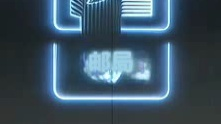
\includegraphics[width=0.3\linewidth]{figs/cells/mg_g117_zh_metal_s1_B1.jpg} & 
\includegraphics[width=0.3\linewidth]{figs/cells/mg_g117_zh_metal_s1_matgen.jpg} \\
&\parbox[t]{0.3\linewidth}{\centering\scriptsize \textcolor{badred}{\ding{55}}\,\texttt{\zh{邮局}}} & \parbox[t]{0.3\linewidth}{\centering\scriptsize \textcolor{okgreen}{\ding{51}}\,\texttt{\zh{邮局}}} & \parbox[t]{0.3\linewidth}{\centering\scriptsize \textcolor{okgreen}{\ding{51}}\,\texttt{\zh{邮局}}} \\[3pt]
\scriptsize farther (LED sign) & 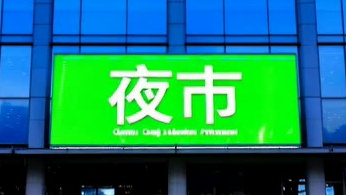
\includegraphics[width=0.3\linewidth]{figs/cells/mg_g085_zh_signboard_s8_orig.jpg} & 
\includegraphics[width=0.3\linewidth]{figs/cells/mg_g085_zh_signboard_s8_B1.jpg} & 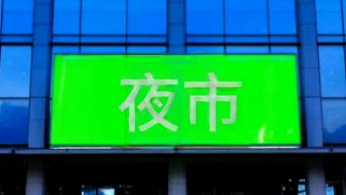
\includegraphics[width=0.3\linewidth]{figs/cells/mg_g085_zh_signboard_s8_matgen.jpg} \\
&\parbox[t]{0.3\linewidth}{\centering\scriptsize \textcolor{badred}{\ding{55}}\,\texttt{\zh{夜市} Qingdao Night Marke}} & \parbox[t]{0.3\linewidth}{\centering\scriptsize \textcolor{okgreen}{\ding{51}}\,\texttt{\zh{夜市}}} & \parbox[t]{0.3\linewidth}{\centering\scriptsize \textcolor{okgreen}{\ding{51}}\,\texttt{\zh{夜市}}} \\[3pt]
\scriptsize unreadable (poster) & 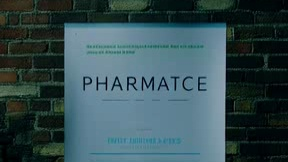
\includegraphics[width=0.3\linewidth]{figs/cells/mg_g025_en_paper_s2_orig.jpg} & 
\includegraphics[width=0.3\linewidth]{figs/cells/mg_g025_en_paper_s2_B1.jpg} & 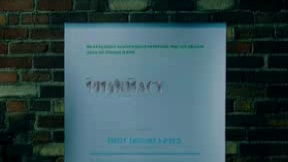
\includegraphics[width=0.3\linewidth]{figs/cells/mg_g025_en_paper_s2_matgen.jpg} \\
&\parbox[t]{0.3\linewidth}{\centering\scriptsize \textcolor{badred}{\ding{55}}\,\texttt{PHARMATCE}} & \parbox[t]{0.3\linewidth}{\centering\scriptsize \textcolor{okgreen}{\ding{51}}\,\texttt{PHARMACY}} & \parbox[t]{0.3\linewidth}{\centering\scriptsize \textcolor{badred}{\ding{55}}\,\texttt{PHARMACY}} \\[3pt]
\end{tabular}
\caption{\textbf{The material generator on real clips} (gate R2; three hand-picked examples; Original / Banksy / generator, with the reader's transcription). Trained only on rendered pairs, the generator keeps the glyphs (their alpha is an input) but writes them with low contrast and desaturated colour on most carriers, which the appearance distance and the reader both penalise; it is closer to the original than Banksy only on metal.}
\label{fig:matgen}
\end{figure}

\paragraph{A glyph-locked material generator.} The appearance gap invites a learned module that keeps \method's glyphs and generates only their material. We built one and registered four gates for it (supplement). Counterfactual pairs rendered in Blender---one scene, material and camera path with two strings, so that only the text differs (2{,}000 training pairs over 8 carrier materials, 5 text styles and 41 fonts; 80 validation pairs with the benchmark's target strings, which training excludes)---train a conditional U-Net in the carrier's UV space that receives the erased background, the target glyph alpha and the other string's rendered material and predicts the text layer; the alpha fixes identity, layout and topology. On held-out pairs the model closes 0.48 of the gap between a flat paste and the rendered truth with a glyph IoU of 0.95, below the registered 0.50; the one registered capacity test (1.8$\times$ the parameters, same data, seed and schedule) closes 0.498. Applied zero-shot to the 129 benchmark clips outside the development sets that both \method and \steer repair (\cref{fig:matgen}), it fails every registered criterion: appearance distance 3.06 against 1.99 for \method (paired $+1.08$, 95\% CI $[+0.73, +1.45]$; closer than \method on 24\% of the clips) and 20 readings lost (84.5\% vs.\ 100\%). Under our registered protocol, increasing model capacity by 1.8$\times$ did not close the synthetic-domain criterion, and zero-shot transfer to generated videos substantially degraded both appearance and readability. A registered photometric ablation with the frozen weights (supplement) attributes part of the transfer loss to the renders' photometry---bright, low-contrast text---and leaves the rest unexplained by it; the calibrated output is still farther from the original than a flat paste of the source's median colour. We stop at the gates. The result bounds this generator, data and recipe, not learned material transfer in general, and the glyph-agnostic appearance distance is insensitive to structure, so improvements it cannot see may exist.
